\documentclass[]{standalone}
\usepackage{alltt}
\usepackage{relsize}
\usepackage{tikz}

\usepackage{subcaption}

\usepackage{amsmath, amssymb}
\usetikzlibrary{shapes,trees}
\usetikzlibrary{positioning,backgrounds}

\renewcommand{\vec}[1]{\mathbf{#1}}
\newcommand{\mat}[1]{\mathbf{#1}}


\newcommand{\rpt}[2][1]{\foreach \n in {1,...,#1}{#2}}

\newcommand{\nnode}[4][0]{\node[rectangle,rounded corners,draw,fill=black!#1](#2)[#3]{$\rpt[#4]{\:\!\circ\:\!}$}}
\newcommand{\weight}[3]{\node[rectangle,rounded corners,dotted,draw,fill=black!5](#1)[#2]{#3}}
\newcommand{\inode}[3]{\nnode{#1}{#2}{3};\weight{#1W}{below =0cm of #1}{#3}}
\newcommand{\ionode}[4]{\nnode{#1I}{#2}{3};\weight{#1WI}{below =0cm of #1I}{#3};\nnode[20]{#1O}{left=0.3cm of #1I}{3};\weight{#1WO}{above =0cm of #1O}{#4};}
\newcommand{\rnode}[3]{\weight{#1W}{#2}{#3};\nnode[20]{#1L}{above left=0cm of #1W.north}{3};\nnode[20]{#1R}{above right=0cm of #1W.north}{3};}
\newcommand{\rnn}[3]{\node(#1)[regular polygon,  regular polygon sides=4, rounded corners, draw, minimum width = 1.5cm, label=below:{#3}][#2]{};}

\begin{document}
\small


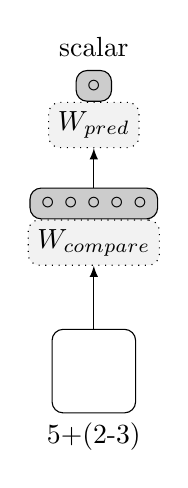
\begin{tikzpicture}[>=latex,node distance = 0.5cm] 

\weight{Wsm}{}{$W_{pred}$};
\nnode[20]{sm}{above =0cm of Wsm}{1};
\node(classes)[above of= sm]{scalar};
\nnode[20]{c}{below = of Wsm}{5};
\weight{Wc}{below=0cm of c}{$W_{compare}$};
\draw[->] (c) -> (Wsm);

\rnn{t}{below = 0.8 of Wc}{5+(2-3)};
\draw[->](t.90)->(Wc);

\end{tikzpicture}


\end{document}
